\section{Video Diffusion Dài hạn: Hướng tới Kể chuyện Bằng Hình ảnh Động}
\label{sec:long_term_video_diffusion}

\subsection{Tổng quan: Thách thức của Thời gian}
\label{subsec:long_video_overview}
Sự thành công của các mô hình Text-to-Video như Sora và Kling đã chứng minh khả năng của AI trong việc tạo ra các đoạn video ngắn, chất lượng cao. Tuy nhiên, việc mở rộng từ vài giây lên vài phút—hay còn gọi là \textbf{sinh video dài hạn (long-term video generation)}—đặt ra một loạt các thách thức hoàn toàn mới và phức tạp hơn rất nhiều.

Vấn đề không chỉ nằm ở gánh nặng tính toán, mà còn ở việc duy trì \textbf{tính nhất quán ngữ nghĩa và tường thuật (semantic and narrative consistency)} trên một khoảng thời gian dài.
\begin{itemize}
	\item Một nhân vật phải giữ nguyên ngoại hình, quần áo, và các đặc điểm nhận dạng.
	\item Một bối cảnh không thể thay đổi đột ngột nếu không có lý do.
	\item Các hành động và sự kiện phải tuân theo một logic nhân quả, tạo thành một câu chuyện có thể hiểu được.
\end{itemize}
Giải quyết những thách thức này đòi hỏi các kiến trúc không chỉ có khả năng mô hình hóa các chuyển động cục bộ, mà còn phải có một "bộ nhớ" và khả năng "lý luận" về các mối quan hệ theo thời gian ở quy mô lớn. Hai trong số những mô hình tiên phong giải quyết bài toán này là Vidu và Runway Gen-3.

\subsection{Vidu (Shengshu Technology \& Tsinghua University, 2024)}
\label{subsec:vidu}
\textbf{Vidu} là mô hình sinh video từ văn bản quy mô lớn đầu tiên của Trung Quốc, được công bố vào tháng 4 năm 2024. Nó có khả năng tạo ra các video dài 16 giây ở độ phân giải 1080p và cho thấy sự hiểu biết sâu sắc về các yếu tố vật lý và văn hóa Trung Quốc.

\textbf{Kiến trúc và Triết lý:}
Vidu được xây dựng dựa trên một kiến trúc lai, kết hợp những ý tưởng tốt nhất từ các mô hình đi trước.
\begin{itemize}
	\item \textbf{Universal Vision Transformer (U-ViT):} Kiến trúc nền tảng của Vidu được cho là dựa trên U-ViT, một sự hợp nhất giữa Vision Transformer và kiến trúc U-Net kinh điển. Điều này cho phép mô hình vừa xử lý hiệu quả các phụ thuộc tầm xa thông qua self-attention, vừa có cấu trúc phân cấp để xử lý các đặc trưng ở các quy mô khác nhau.
	\item \textbf{Diffusion Transformer (DiT):} Tương tự như Sora, Vidu sử dụng một kiến trúc dựa trên Transformer để thực hiện quá trình khử nhiễu trong không gian tiềm ẩn.
	\item \textbf{Mô hình hóa Thời gian Dài hạn:} Vidu tập trung vào việc mô hình hóa các chuyển động phức tạp và duy trì tính nhất quán bằng cách xử lý đồng thời một số lượng lớn các khung hình trong quá trình huấn luyện, giúp nó học được các quy luật động học và tường thuật phức tạp.
\end{itemize}
Sự ra đời của Vidu cho thấy một xu hướng toàn cầu trong việc xây dựng các mô hình video nền tảng và khẳng định tầm quan trọng của các kiến trúc lai (Transformer + CNN) trong việc đạt được sự cân bằng giữa hiệu quả và khả năng mô hình hóa mạnh mẽ.

\subsection{Runway Gen-3 Alpha (Runway, 2024)}
\label{subsec:runway_gen3}
\textbf{Runway}, một trong những công ty khởi nghiệp tiên phong trong lĩnh vực AI sáng tạo, đã liên tục đẩy ranh giới của việc sinh video. Phiên bản mới nhất của họ, \textbf{Gen-3 Alpha} (công bố tháng 6 năm 2024), đại diện cho một bước tiến đáng kể trong việc kiểm soát chi tiết và tính nhất quán của nhân vật.

\textbf{Kiến trúc và Các Cải tiến:}
Gen-3 được huấn luyện trên một kiến trúc đa phương thức (multimodal) thế hệ mới, được xây dựng dựa trên sự hợp tác giữa các nhà nghiên cứu và nghệ sĩ.
\begin{itemize}
	\item \textbf{Mô hình Nền tảng Đa phương thức:} Gen-3 được huấn luyện để hiểu và tạo ra nội dung từ sự kết hợp của văn bản, hình ảnh và video. Điều này cho phép nó tạo ra các video không chỉ dựa trên prompt văn bản, mà còn có thể bắt đầu từ một ảnh tham chiếu và "hoạt hóa" nó một cách nhất quán.
	\item \textbf{Kiểm soát Chi tiết và Nhất quán Nhân vật:} Một trong những điểm nhấn lớn nhất của Gen-3 là khả năng tạo ra các nhân vật con người với các biểu cảm, hành động và phong cách cực kỳ chi tiết và duy trì sự nhất quán của họ qua các cảnh quay phức tạp.
	\item \textbf{Các Công cụ Điều khiển Nâng cao:} Runway cung cấp một bộ công cụ cho phép các nhà sáng tạo kiểm soát chi tiết quá trình sinh, bao gồm:
	\begin{itemize}
		\item \textbf{Motion Brush:} "Vẽ" chuyển động lên một vùng cụ thể của ảnh tĩnh.
		\item \textbf{Camera Controls:} Kiểm soát chính xác chuyển động của camera (zoom, pan, tilt).
		\item \textbf{Director Mode:} Cho phép điều khiển sâu hơn về mặt thẩm mỹ và tường thuật.
	\end{itemize}
\end{itemize}
Runway Gen-3 không chỉ là một mô hình sinh video, mà là một "xưởng phim AI" (AI film studio), cung cấp các công cụ chuyên nghiệp để kiểm soát quá trình sáng tạo, thu hẹp khoảng cách giữa các mô hình nghiên cứu và các công cụ sản xuất thực tế.

\begin{center}
	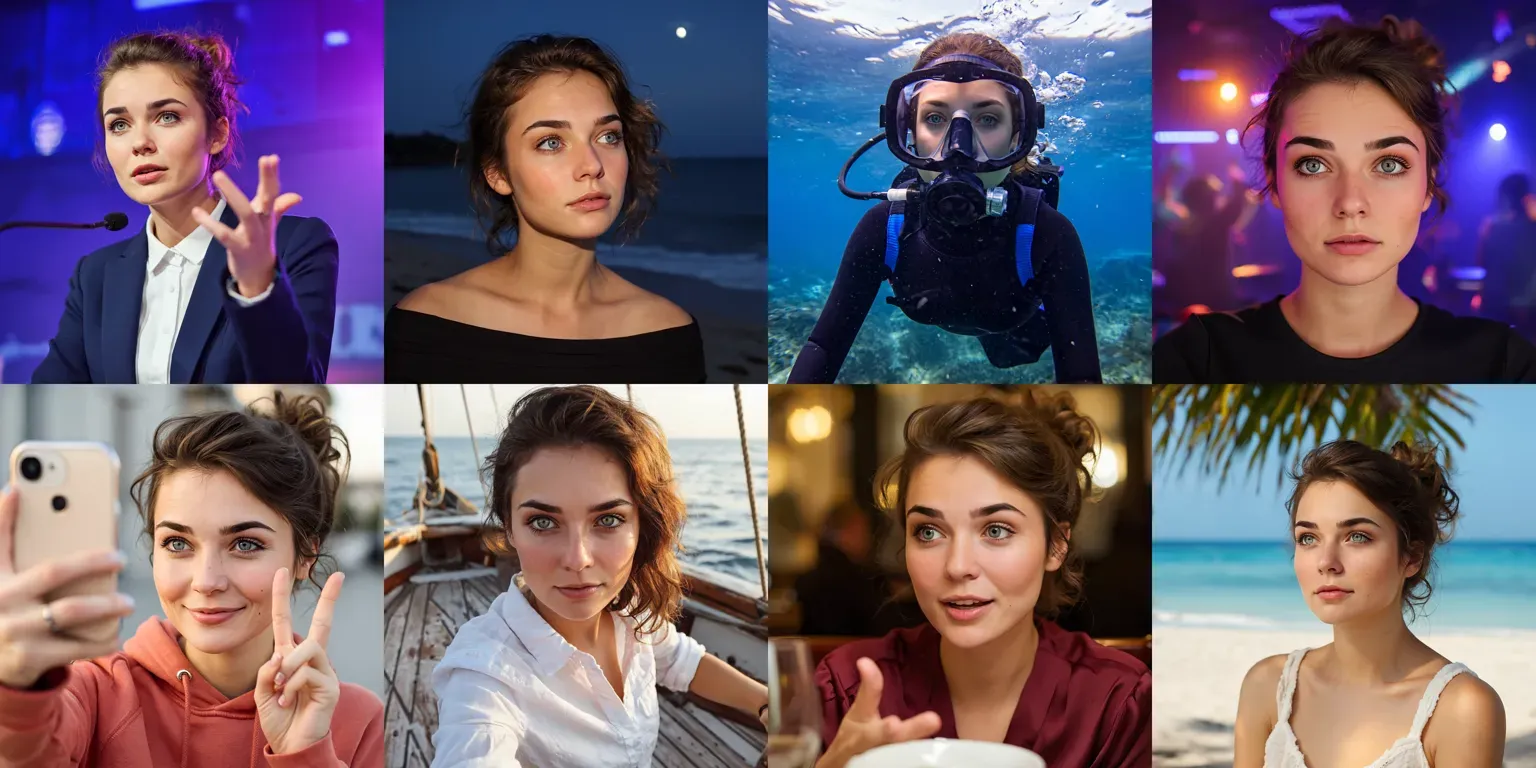
\includegraphics[width=1.0\textwidth]{images/runway_gen3_character_consistency.png}
	\captionof{figure}{Ví dụ về tính nhất quán của nhân vật trong Runway Gen-3. Mô hình có thể tạo ra cùng một nhân vật trong các bối cảnh và hành động khác nhau, một thách thức lớn trong sinh video dài hạn.}
	\label{fig:runway_gen3_consistency}
\end{center}
% Keyword gợi ý: runway gen 3 character consistency, generative video models

\subsection{Kết luận: Hướng tới các "Cỗ máy Kể chuyện" AI}
\label{subsec:long_video_conclusion}
Các mô hình sinh video dài hạn như Vidu và Runway Gen-3 đang biến khoa học viễn tưởng thành hiện thực. Chúng đại diện cho một bước tiến từ việc tạo ra các "clip" ngắn, rời rạc sang việc tạo ra các "cảnh quay" (scenes) có cấu trúc, nhất quán và có khả năng kể chuyện.

Đây không chỉ là một bước tiến về mặt kỹ thuật, mà còn là một sự thay đổi mô thức trong cách chúng ta tạo ra nội dung số:
\begin{itemize}
	\item \textbf{Từ Ảnh tĩnh sang Thế giới Động:} Các mô hình này đang học cách mô phỏng các quy luật vật lý, động học và tương tác, biến chúng thành các "mô hình thế giới" thu nhỏ.
	\item \textbf{Từ Lệnh sang Hợp tác:} Quá trình sáng tạo không còn là một lệnh "text-to-video" một chiều. Với các công cụ điều khiển tương tác, nó đang trở thành một cuộc đối thoại, một quá trình hợp tác giữa người sáng tạo và AI.
	\item \textbf{Dân chủ hóa Sản xuất Phim:} Các công cụ này hứa hẹn sẽ hạ thấp đáng kể rào cản kỹ thuật và tài chính trong việc sản xuất video, cho phép các nghệ sĩ và nhà sáng tạo độc lập có thể hiện thực hóa những ý tưởng mà trước đây chỉ có các xưởng phim lớn mới có thể làm được.
\end{itemize}
Trong giai đoạn 2024–2025 và xa hơn, chúng ta sẽ chứng kiến sự phát triển nhanh chóng của các \textbf{Mô hình Video Nền tảng (Video Foundation Models)}, với khả năng tạo ra các video ngày càng dài hơn, phức tạp hơn và có khả năng tương tác cao hơn. Đây là nền tảng cho một kỷ nguyên mới của truyền thông, giải trí, và nghệ thuật, nơi ranh giới giữa thực và ảo, giữa người và máy, ngày càng trở nên mờ nhạt.

\section*{Tài liệu tham khảo}
\begin{itemize}
	\item[1] Shengshu Technology \& Tsinghua University. (2024). \textit{Vidu: A Large-Scale Text-to-Video Generation Model}. Technical Report. (Công bố mô hình Vidu).
	\item[2] Runway. (2024). \textit{Introducing Gen-3 Alpha: A New Frontier for Video Generation}. RunwayML Blog. (Công bố mô hình Runway Gen-3 Alpha).
	\item[3] OpenAI. (2024). \textit{Video generation models as world simulators}. OpenAI Technical Report. (Báo cáo kỹ thuật về Sora, đặt nền móng cho các mô hình video quy mô lớn).
	\item[4] Esser, P., et al. (2023). \textit{Structure and Content-Guided Video Synthesis with Diffusion Models}. Runway Research. (Một ví dụ về các công trình nghiên cứu nền tảng của Runway).
	\item[5] Wang, Z., et al. (2023). \textit{U-ViT: A Unified Vision Transformer for Visual Recognition and Generation}. (Bài báo giới thiệu kiến trúc U-ViT, một hướng tiếp cận lai có thể là nền tảng cho Vidu).
\end{itemize}